\documentclass[11pt]{article}

% Packages
\usepackage[utf8]{inputenc}
\usepackage[T1]{fontenc}
\usepackage{amsmath, amssymb, amsthm}
\usepackage{graphicx}
\usepackage{booktabs}
\usepackage{hyperref}
\usepackage{cleveref}
\usepackage{xcolor}
\usepackage{enumitem}
\usepackage{algorithm}
\usepackage{algorithmic}
\usepackage{multirow}
\usepackage{geometry}
\usepackage{natbib}
\usepackage{microtype}
\usepackage{float}
\usepackage[section]{placeins}
\usepackage{array}
\usepackage{ragged2e}

\geometry{margin=0.92in}
\definecolor{Accent}{HTML}{1F4E79}
\definecolor{AccentLight}{HTML}{EEF5FA}
\hypersetup{colorlinks=true, linkcolor=Accent, citecolor=Accent, urlcolor=Accent, pdfauthor={David Vesterlund}, pdftitle={Grokking the Discrete Logarithm: Scaling Across Model Capacity and Mechanistic Analysis}}
\setlength{\parindent}{0pt}
\setlength{\parskip}{0.42em}
\setlist[itemize]{topsep=0.35em,itemsep=0.18em,parsep=0pt}
\setlist[enumerate]{topsep=0.35em,itemsep=0.25em,parsep=0pt}
\renewcommand{\arraystretch}{1.12}

% Theorem environments
\newtheorem{theorem}{Theorem}
\newtheorem{lemma}{Lemma}
\newtheorem{proposition}{Proposition}
\newtheorem{definition}{Definition}
\newtheorem{remark}{Remark}

% Custom commands
\newcommand{\Fp}{\mathbb{F}_p}
\newcommand{\Fps}{\mathbb{F}_p^*}
\newcommand{\Z}{\mathbb{Z}}
\newcommand{\R}{\mathbb{R}}
\newcommand{\Tmem}{T_{\mathrm{mem}}}
\newcommand{\Tgrok}{T_{\mathrm{grok}}}
\newcommand{\Tfifty}{T_{50}}
\newcommand{\Tninety}{T_{90}}
\newcommand{\Tninfive}{T_{95}}
\newcommand{\Tnine}{T_{99}}
\newcommand{\Gdelay}{G}
\newcommand{\wdmax}{\mathrm{wd}_{\max}}
\newcommand{\Pcore}{P_{\mathrm{core}}}
\newcommand{\Ptotal}{P_{\mathrm{total}}}
\newcommand{\dmodel}{d_{\mathrm{model}}}
\newcommand{\nheads}{n_{\mathrm{heads}}}
\newcommand{\nlayers}{n_{\mathrm{layers}}}
\newcommand{\Ncrit}{N_{\mathrm{crit}}}
\newcommand{\Cgrok}{C_{\mathrm{grok}}}

% Title
\title{\textbf{Grokking the Discrete Logarithm:\\
Scaling Across Model Capacity and Mechanistic Analysis}}
\author{
David Vesterlund \\
Industrial Research at Vesterlund Ventures Holding AB
}
\date{}

\begin{document}

\maketitle

\begin{abstract}
To the best of our knowledge, we provide the first systematic demonstration that a transformer can exhibit grokking on the full \emph{variable-base} finite-field discrete logarithm mapping, $(g,h)\mapsto x$ with $g^x\equiv h\pmod p$. A 427k-parameter, two-layer transformer reaches 99.8\% test accuracy at $p=113$ only after a long memorization phase, giving a clear instance of delayed algorithmic generalization on a structured inverse problem. We then perform a 12-model capacity sweep spanning 90k--14.4M parameters. Grokking is observed at the 427k anchor and again from 1.64M through 14.4M parameters under a staged training-data schedule, with a non-monotonic region whose outcome changes when training data are increased. Mechanistically, the grokking transition is accompanied by increasing alignment with multiplicative-character structure. Symbolic regression on hidden states preferentially recovers character-aligned trigonometric features, while a free operator set independently recovers Fourier harmonics. Finally, prime-order and disjoint-generator controls show that the phenomenon is not restricted to smooth composite-order groups or to generators seen during training. These results position DLP as a compact benchmark for studying how memorization, representation formation, and generalization interact across neural scale.
\end{abstract}

\begin{center}
\fcolorbox{Accent}{AccentLight}{%
\begin{minipage}{0.94\linewidth}
\small
\textbf{Key results.}\quad
\textbf{(1)} To the best of our knowledge, this is the first systematic grokking study of the full variable-base DLP mapping.\;
\textbf{(2)} A 427k-parameter transformer reaches 99.8\% test accuracy only after prolonged memorization.\;
\textbf{(3)} A 12-model sweep from 90k to 14.4M parameters shows DLP grokking across multiple neural scales, with a data-dependent non-monotonic region.\;
\textbf{(4)} Spectral and symbolic analyses identify multiplicative-character/Fourier structure, while prime-order and generator-OOD controls preserve successful generalization.
\end{minipage}}
\end{center}
\vspace{0.35em}

% ============================================================================
% 1. INTRODUCTION
% ============================================================================

\section{Introduction}
\label{sec:intro}

The \emph{grokking} phenomenon \citep{power2022grokking}---in which a neural network abruptly transitions from memorization to generalization long after overfitting---has emerged as a powerful lens for studying representation learning. While initially observed on modular arithmetic tasks (addition, multiplication, permutation composition), the phenomenon has been studied extensively through mechanistic interpretability \citep{nanda2023progress}, effective theories of representation learning \citep{liu2022understanding}, circuit efficiency \citep{varma2023explaining}, and the slingshot mechanism \citep{thilak2022slingshot}.

Prior grokking work has largely focused on forward algebraic operations such as modular addition and multiplication, where the target map is directly specified by a simple group operation. The discrete logarithm problem (DLP)---given a generator $g$ of $\Fps$ and an element $h \in \Fps$, find $x$ such that $g^x \equiv h \pmod{p}$---is qualitatively different: it is an \emph{inverse} map on a cyclic group, and no polynomial-time classical algorithm is known for generic groups of large prime order. However, DLP provides an excellent \emph{learning benchmark} because it combines highly structured algebra (the cyclic group $\Fps$) with a nontrivial inverse mapping that has no simple local input-output rule.

To the best of our knowledge, this is the first systematic study demonstrating grokking on the full variable-base discrete logarithm mapping, complementing prior work in which discrete-log coordinates arise as an internal representation for modular multiplication. \citet{takhanov2024intractability} showed that gradient-based methods provably cannot efficiently learn the parity bit of the discrete logarithm in cyclic groups of large prime order; our experiments use small finite groups and make no claims about practical cryptanalysis.

In this work, we make the following contributions:

\begin{enumerate}[leftmargin=*]
    \item \textbf{First full-DLP grokking benchmark (to our knowledge).} A two-layer, 427k-parameter transformer groks the variable-base map $(g,h)\mapsto x$ at $p=113$, reaching 99.8\% held-out accuracy after a pronounced memorization plateau (\Cref{sec:discovery}).

    \item \textbf{Scaling across neural capacity.} We run a 12-model sweep from 90k to 14.4M parameters. Grokking occurs at multiple model scales, while an intermediate non-monotonic region is sensitive to the amount of training data (\Cref{sec:scaling}).

    \item \textbf{Training dynamics and mechanistic signatures.} The anchor model exhibits a five-stage trajectory with repeated slingshot events, and its hidden representation becomes increasingly aligned with multiplicative-character structure during generalization (\Cref{sec:dynamics,sec:mechanistic}).

    \item \textbf{Symbolic regression of hidden states.} Algebra-aware symbolic regression preferentially fits character-aligned trigonometric features, while free regression independently recovers valid Fourier harmonics without access to modular features (\Cref{sec:symbolic}).

    \item \textbf{Structural controls.} DLP also groks in a prime-order subgroup, and a disjoint-generator split reaches 100\% test accuracy, showing generalization beyond generators seen during training (\Cref{sec:prime_order}).
\end{enumerate}

% ============================================================================
% 2. DLP LEARNING BENCHMARK
% ============================================================================

\section{DLP Learning Benchmark}
\label{sec:benchmark}

\subsection{Task Definition}

We study the \emph{variable-base} discrete logarithm problem. Given a prime $p$, the model receives a generator $g$ drawn uniformly from the set of primitive roots of $\Fps$ and an element $h \in \Fps$, and must predict the discrete logarithm $x \in \{0, \ldots, p-2\}$ such that:
\begin{equation}
    g^x \equiv h \pmod{p}, \qquad (g, h) \mapsto x.
\end{equation}
The model predicts $x$ as a classification target over $p - 1$ classes. The input is tokenized as $[\mathrm{BOS}, g, \mathrm{SEP}, h, \mathrm{EOS}]$ where $g$ and $h$ are encoded as integer tokens.

The full primitive-generator domain for prime $p$ has size:
\begin{equation}
    |\text{domain}| = \varphi(p-1) \times (p - 1),
\end{equation}
where $\varphi$ is Euler's totient function (counting primitive roots) and $p - 1$ is the group order (number of possible $x$ values per generator). For $p = 113$, this gives $\varphi(112) \times 112 = 48 \times 112 = 5{,}376$ unique $(g, h, x)$ triples. At a train fraction $\rho = 0.30$, the training set has 1,612 examples and the test set has 3,764 examples, with no overlap between train and test $(g, h)$ pairs.

\subsection{Architecture}

We use a \emph{GrokkingTransformer}: a standard transformer encoder with pre-norm (LayerNorm before attention and FFN), GELU activations, and learned positional embeddings. The architecture is:
\begin{equation}
    \mathbf{h} = \mathrm{Dropout}(\mathrm{Embed}(\mathbf{t}) + \mathrm{PosEmbed}(\mathbf{p}))
    \xrightarrow{\text{$L$ layers}} \mathbf{h}'
    \xrightarrow{\text{Unembed}} \hat{\mathbf{y}}
\end{equation}
where each layer is a pre-norm TransformerEncoderLayer \citep{vaswani2017attention} with $\dmodel$ dimensions, $\nheads$ attention heads, and FFN dimension $4 \cdot \dmodel$.

The primary model (M04) has $\dmodel = 128$, $\nheads = 4$, $\nlayers = 2$, yielding $\Ptotal = 427{,}253$ parameters ($\Pcore = 396{,}544$ excluding embeddings and unembedding). The model grid spans M01--M12 with $\dmodel$ from 56 to 768 (\Cref{tab:model_grid}).

\subsection{Training}

\paragraph{Optimizer.} AdamW \citep{loshchilov2019decoupled} with learning rate $\eta = 10^{-3}$, $\beta_1 = 0.9$, $\beta_2 = 0.999$, and weight decay $\lambda$ applied via the decoupled formulation. Full-batch training (no mini-batching for $p = 113$).

\paragraph{Progressive Weight Decay Schedule.} Weight decay follows a progressive ramp schedule:
\begin{equation}
    \lambda(t) = \begin{cases}
        \lambda_{\mathrm{start}} & \text{if } t < \Tmem \\
        \min\!\left(\lambda_{\mathrm{start}} + \Delta\lambda \cdot \left\lfloor\frac{t - \Tmem}{\Delta t_{\mathrm{ramp}}}\right\rfloor,\ \wdmax\right) & \text{if } t \geq \Tmem
    \end{cases}
    \label{eq:wd_schedule}
\end{equation}
where $\lambda_{\mathrm{start}} = 0.05$, $\Delta\lambda = 0.05$, $\Delta t_{\mathrm{ramp}} = 1000$ epochs, and $\wdmax = 0.30$. The ramp begins only after the model achieves $>99\%$ train accuracy ($\Tmem$), and increases by 0.05 every 1000 epochs until reaching $\wdmax = 0.30$. The learning rate is held constant ($\eta = 10^{-3}$) throughout training.

\paragraph{Weight Decay Auto-Scaling.} For models of different sizes, $\wdmax$ is scaled based on core parameter count:
\begin{equation}
    \wdmax = \min\!\left(0.30,\ 0.30 \cdot \sqrt{\frac{393\text{k}}{\Pcore}}\right)
    \label{eq:wd_auto}
\end{equation}
This \emph{decreases} $\wdmax$ for larger models (which have more capacity for memorization and thus need less regularization pressure to eventually favor generalization). For M04 ($\Pcore = 396.5\text{k}$), this yields $\wdmax \approx 0.30$. We treat WD as a controlled scaling variable and report it explicitly for each experiment.

\paragraph{Early Stopping.} Training stops when test accuracy exceeds 0.99 for 100 consecutive evaluations (eval interval = 10 epochs).

\subsection{Evaluation Metrics}

We define the following milestones:
\begin{itemize}[leftmargin=*]
    \item $\Tmem$: first epoch where train accuracy $> 99\%$
    \item $\Tfifty$: first epoch where test accuracy $> 50\%$
    \item $\Tninety$: first epoch where test accuracy $> 90\%$
    \item $\Tninfive$: first epoch where test accuracy $> 95\%$
    \item $\Tnine$: first epoch where test accuracy $> 99\%$
    \item $\Gdelay = \Tninety / \Tmem$: grokking delay ratio
\end{itemize}

For scaling comparisons, we report milestones in both epochs and example presentations ($N_{\mathrm{train}} \times \text{epochs}$), since epochs are not comparable across different dataset sizes.


% ============================================================================
% 3. DISCOVERY OF DLP GROKKING
% ============================================================================

\section{Discovery of DLP Grokking}
\label{sec:discovery}

\subsection{L6 Groks at $p = 113$}

The anchor M04 model (427k parameters, $\dmodel=128$, $L=2$) groks the variable-base DLP at $p=113$ with a 30\% training fraction. This anchor run is distinct from the later capacity-sweep runs, which use the training fractions listed in \Cref{tab:model_grid}. \Cref{fig:training_curves} shows the training and test accuracy curves over 37,481 epochs.

\begin{figure}[H]
    \centering
    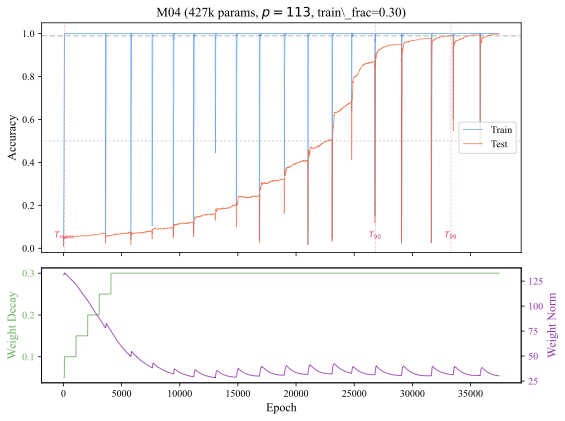
\includegraphics[width=\textwidth]{figures/fig1_training_curves.png}
    \caption{Training curves for M04 ($p = 113$, $\rho = 0.30$, seed 42). \textbf{Top:} Train and test accuracy. The model memorizes at epoch 90, remains at chance test accuracy for $\sim$22k epochs, then groks to 99.8\% by epoch 37k. \textbf{Bottom:} Weight decay schedule (progressive ramp from 0.05 to 0.30) and weight norm (decreasing from 148 to 30 post-grokking).}
    \label{fig:training_curves}
\end{figure}

Key milestones for M04 (seed 42):
\begin{center}
\begin{tabular}{lrlr}
\toprule
Metric & Value & Metric & Value \\
\midrule
$\Tmem$ & 90 & $\Tninety$ & 26,830 \\
$\Tfifty$ & 22,650 & $\Tninfive$ & 28,870 \\
$\Tnine$ & 33,320 & Best test acc & 0.9981 \\
$\Gdelay$ & 298 & Final $\|w\|$ & 30.2 \\
\bottomrule
\end{tabular}
\end{center}

The grokking delay $\Gdelay \approx 298$ is substantial---the model requires $\sim$300$\times$ more training steps to generalize than to memorize. This is consistent with grokking delays observed in modular addition \citep{power2022grokking}, but notable given that DLP is an inverse problem with no trivial local solution rule.


% ============================================================================
% 4. CAPACITY × DATA PHASE DIAGRAM
% ============================================================================

\section{Scaling Across Model Capacity}
\label{sec:scaling}

\subsection{Twelve-Model Capacity Sweep}

We define a model grid spanning M01--M12 with $\dmodel$ from 56 to 768 (\Cref{tab:model_grid}). All models use $L = 2$ layers and are trained on $p = 113$ with the progressive WD schedule.

\begin{table}[H]
\centering
\caption{Model grid for the capacity scaling sweep. All models use $L = 2$ transformer layers, $p = 113$. $\Pcore$ excludes embedding and unembedding parameters. Results from LUMI-G (MI250X). $\Tmem$, $\Tninety$, $\Tnine$ are epochs to $>99\%$ train, $>90\%$ test, $>99\%$ test accuracy. ``---'' indicates the milestone was not reached. Example presentations = $N_{\mathrm{train}} \times \Tninety$.}
\label{tab:model_grid}
\small
\resizebox{\textwidth}{!}{%
\begin{tabular}{lrrrrrrrrr}
\toprule
Model & $\dmodel$ & $\nheads$ & $\Ptotal$ & Train\% & Best Acc & $\Tmem$ & $\Tninety$ & $\Tnine$ & ExPres$\times10^6$ \\
\midrule
M01 & 56 & 2 & 90,221 & 33\% & 7.6\% & 420 & --- & --- & --- \\
M02 & 80 & 4 & 174,917 & 33\% & 11.9\% & 150 & --- & --- & --- \\
M03 & 104 & 4 & 287,261 & 33\% & 15.5\% & 120 & --- & --- & --- \\
\textbf{M04} & \textbf{128} & \textbf{4} & \textbf{427,253} & \textbf{33\%} & \textbf{96.2\%} & \textbf{90} & \textbf{467,720} & \textbf{---} & \textbf{754} \\
M05 & 160 & 5 & 656,917 & 33\% & 25.7\% & 80 & --- & --- & --- \\
M06 & 208 & 8 & 1,093,573 & 33\% & 28.5\% & 60 & --- & --- & --- \\
M07 & 256 & 8 & 1,640,821 & 35\% & 99.8\% & 100 & 652,450 & 678,600 & 1,224 \\
M08 & 320 & 10 & 2,542,517 & 40\% & 99.8\% & 100 & 420,150 & 451,500 & 903 \\
M09 & 384 & 12 & 3,640,821 & 45\% & 99.7\% & 100 & 372,450 & 405,000 & 813 \\
M10 & 480 & 15 & 5,656,917 & 50\% & 99.5\% & 100 & 236,850 & 289,400 & 636 \\
M11 & 608 & 19 & 9,033,173 & 55\% & 99.2\% & 100 & 226,500 & 247,500 & 660 \\
M12 & 768 & 24 & 14,359,413 & 60\% & 99.8\% & 100 & 121,900 & 145,650 & 395 \\
\bottomrule
\end{tabular}%
}
\end{table}

\begin{figure}[H]
    \centering
    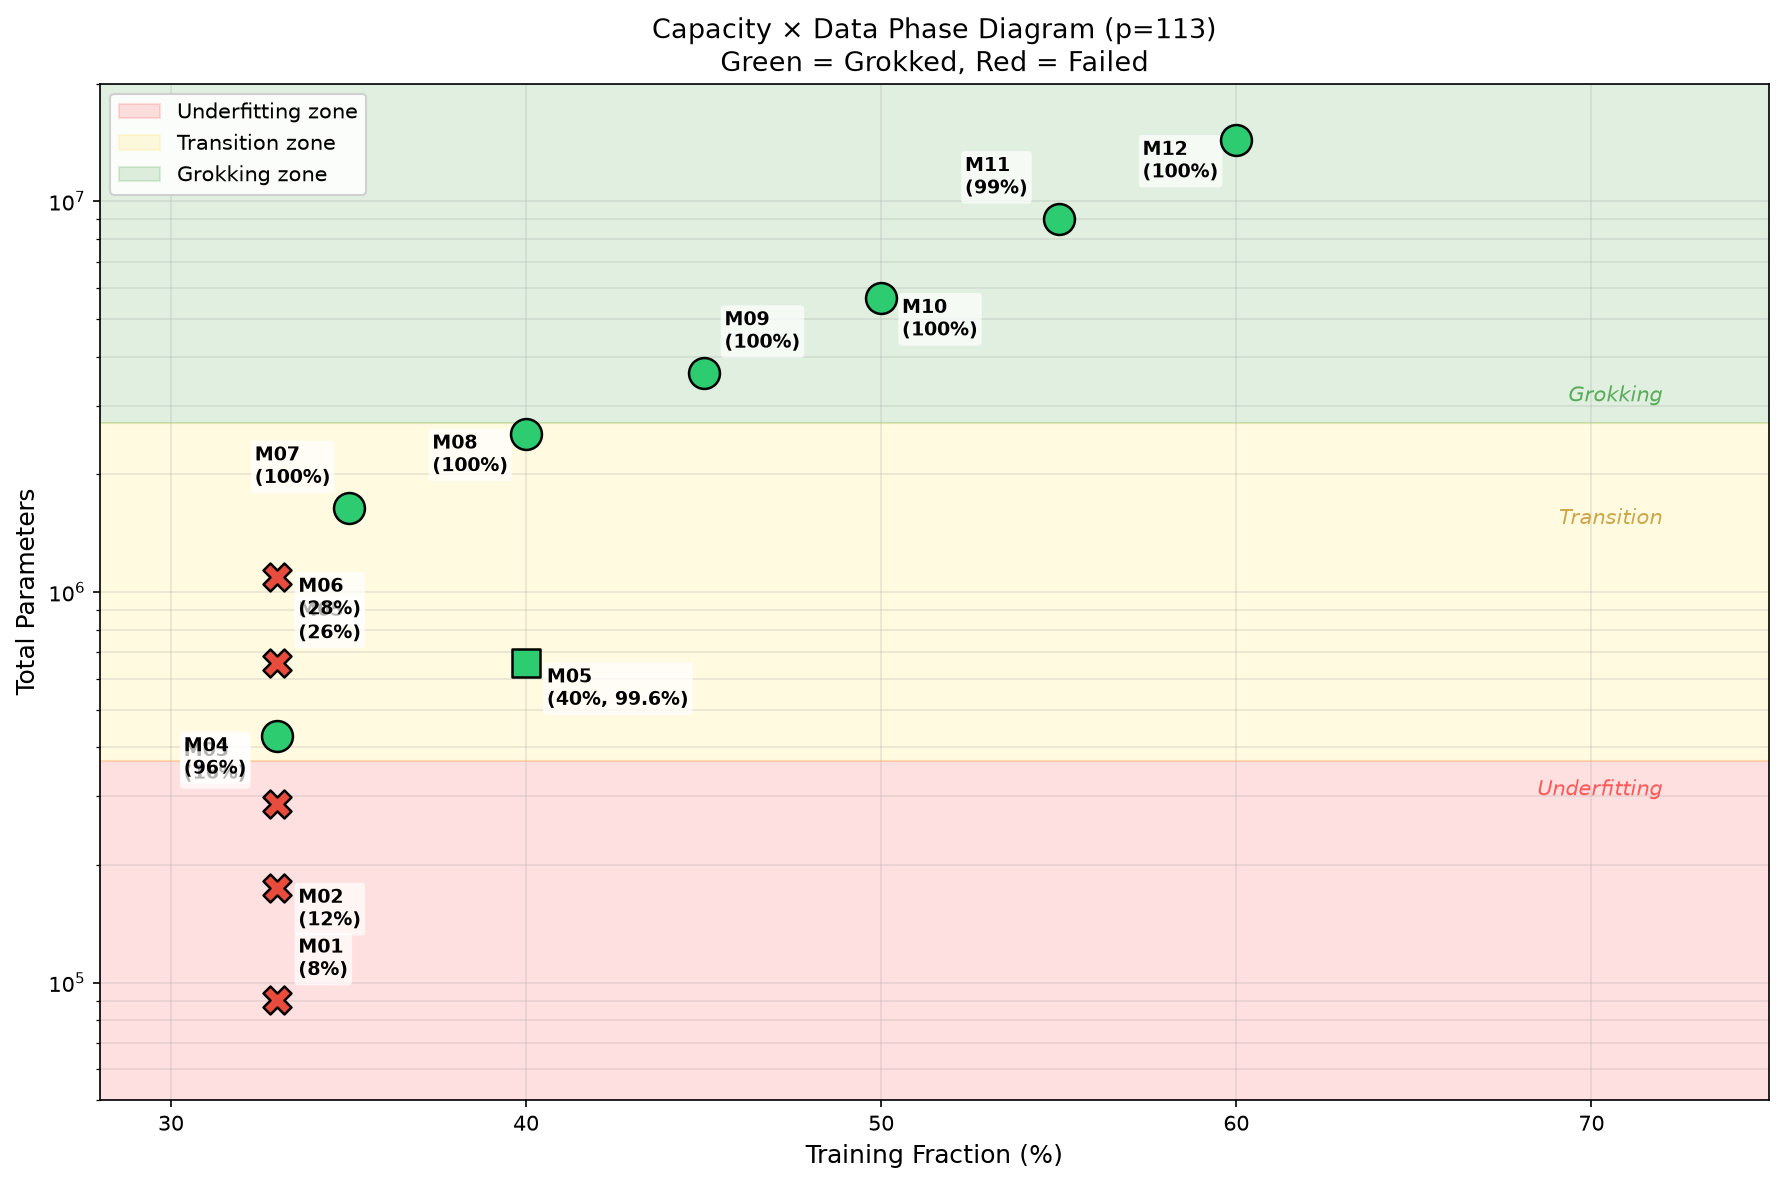
\includegraphics[width=0.86\textwidth]{figures/fig_phase_diagram.png}
    \caption{Empirical capacity--data map ($p=113$). Each point is one model at its training fraction; because training fraction varies across the sweep, the shaded regions are descriptive rather than fitted phase boundaries. Green circles = grokked, red crosses = failed. The M05 point at 40\% (local run) shows the non-monotonicity is train-fraction dependent. Shaded regions indicate approximate zones: red = underfitting, yellow = transition, green = grokking.}
    \label{fig:phase_diagram}
\end{figure}

\subsection{Non-Monotonic Capacity Dependence}

A striking feature of the sweep is a non-monotonic region around M05--M06. M04 (427k parameters) reaches 96.2\% at 33\% training data, while M05 (657k) and M06 (1.09M) remain at 25.7\% and 28.5\%, respectively. Grokking reappears at M07 (1.64M), after which M07--M12 all reach at least 99.2\% under the staged data schedule. Because the training fraction is not fixed across the full sweep, we treat this as an empirical scaling map rather than a one-variable capacity law.

We interpret this as a possible \emph{capacity-dependent sample-complexity frontier}: models in the M05--M06 range may require more training data to grok, and the 33\% fraction used in the initial sweep was insufficient. Supporting this interpretation, a local experiment shows that M05 \emph{does grok} at 99.6\% test accuracy when given 40\% training data (18,321 epochs). The recovery of M05 at a higher training fraction suggests that the non-monotonicity is at least partly data-dependent. We therefore interpret the sweep as evidence for an interaction between model capacity and sample availability, not as evidence for a fixed ``capacity valley.

For M07--M12, we increase the training fraction (35\%--60\%) to compensate. All larger models grok, with grokking time \emph{decreasing} with model size: M12 (14.4M params) groks in 151k epochs, compared to M07's 687k epochs.

\begin{figure}[H]
    \centering
    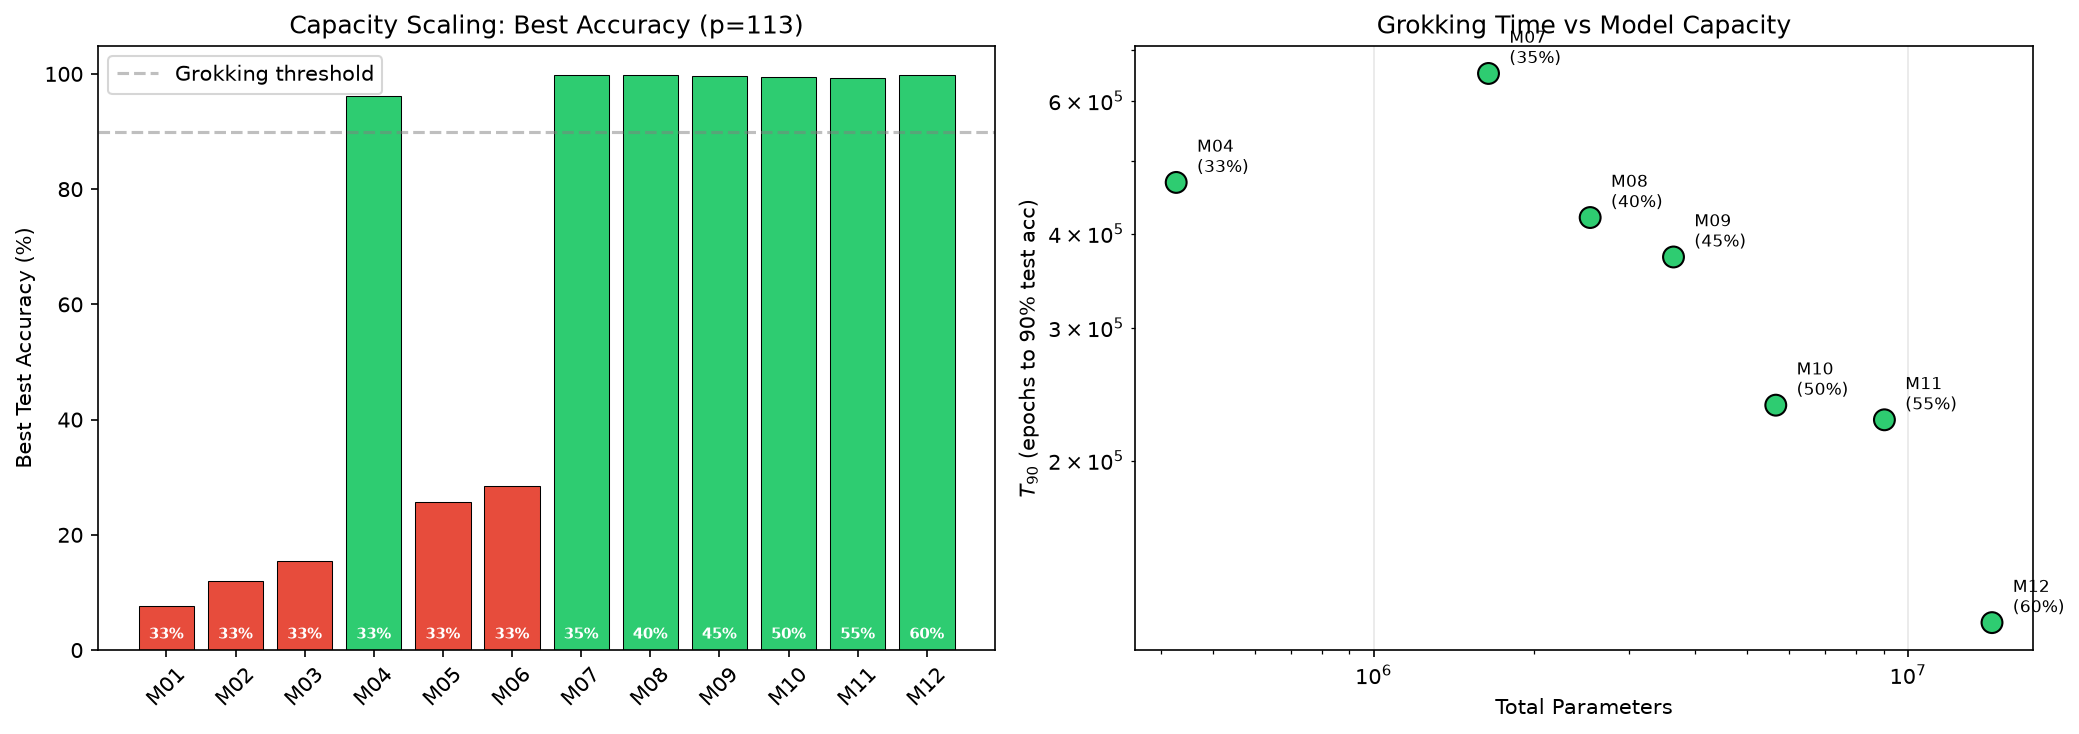
\includegraphics[width=0.96\textwidth]{figures/fig_capacity_scaling.png}
    \caption{Capacity scaling results from LUMI-G. \textbf{Left:} Best test accuracy by model size. Green = grokked ($\geq 90\%$), red = failed. Numbers above bars indicate train fraction. \textbf{Right:} $T_{90}$ vs total parameters (log-log). Grokking time decreases with model size for M07--M12.}
    \label{fig:lumi_capacity}
\end{figure}

\paragraph{Data dependence.}
The capacity sweep already indicates that data availability materially changes whether a model reaches the grokking regime: M05 fails at 33\% training data in the sweep but succeeds in a separate 40\% run. We therefore treat matched sample-complexity estimation as a separate confirmatory study rather than folding pilot data into the present scaling claim.

% ============================================================================
% 5. PROBLEM-SIZE EXTENSION
% ============================================================================

\section{Problem-Size Extension}
\label{sec:group_scaling}

As a preliminary extension beyond $p = 113$, we verified that DLP grokking is not specific to a single prime. On LUMI-G, a model with $\dmodel = 256$ (M14, 2 layers) grokked $p = 521$ at 99.93\% test accuracy (epoch 30,100), demonstrating that the phenomenon extends to primes an order of magnitude larger. We report this only as an extension check, not as a problem-size scaling law: the main paper focuses on the model-capacity and mechanistic results at $p=113$.

% ============================================================================
% 6. TRAINING DYNAMICS ACROSS SCALE
% ============================================================================

\section{Training Dynamics of the Anchor Model}
\label{sec:dynamics}

\subsection{Five-Phase Training Dynamics}

\Cref{fig:five_phases} shows five distinct phases of DLP grokking for M04:

\begin{figure}[H]
    \centering
    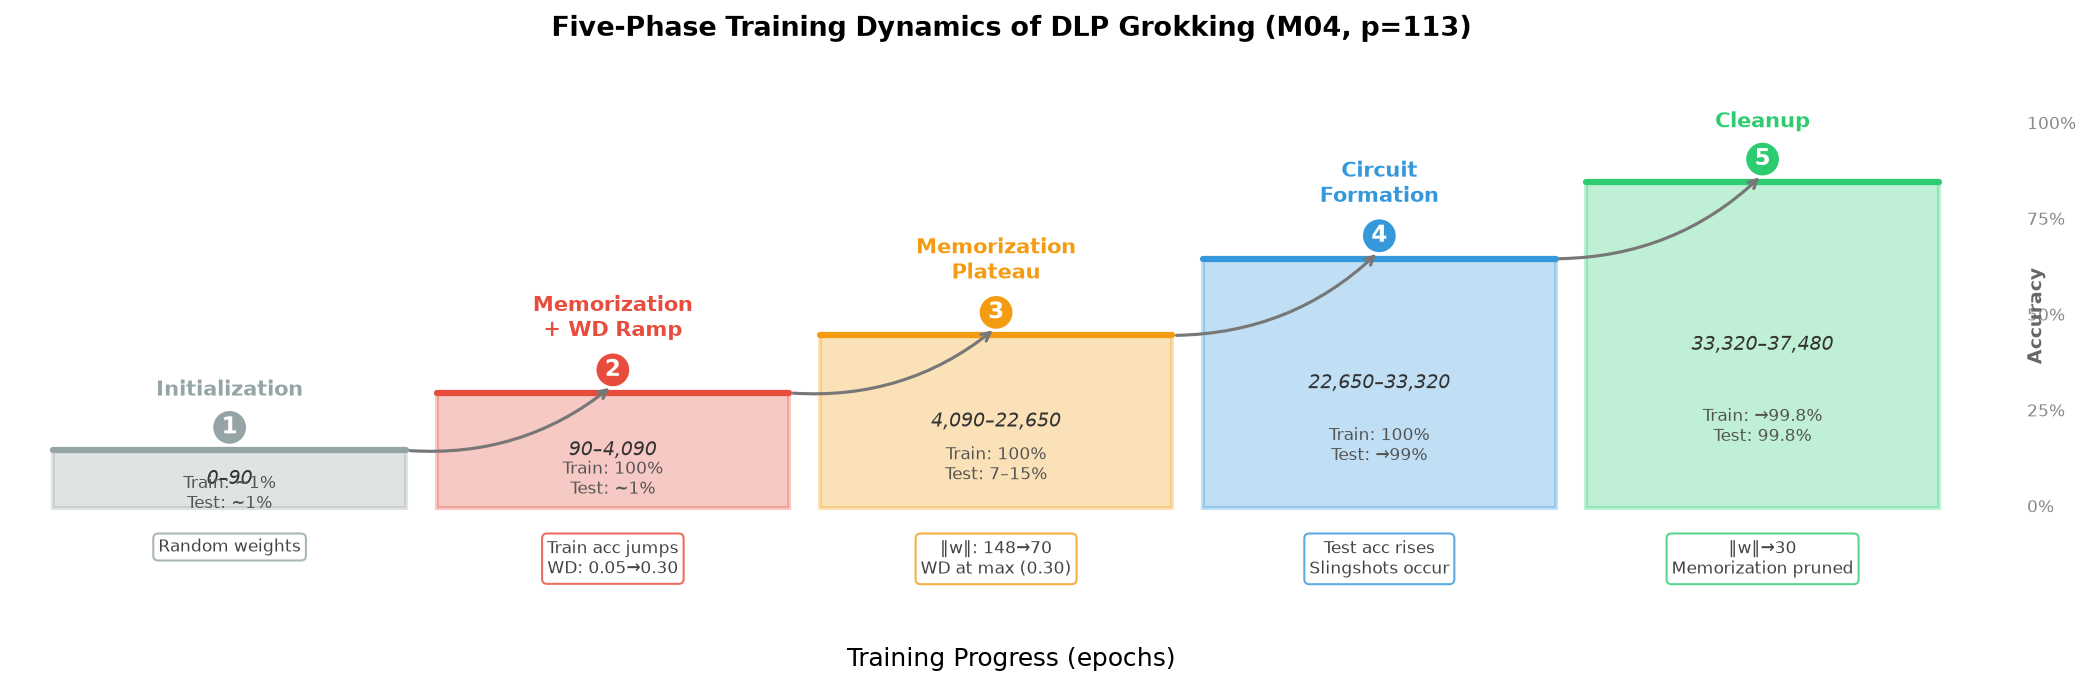
\includegraphics[width=0.95\textwidth]{figures/fig_five_phases.png}
    \caption{Five phases of DLP grokking (M04). A schematic ``stepping board'' view showing the progression from random initialization through memorization, plateau, circuit formation, and cleanup. Each step shows the dominant accuracy behavior and key event. Compare with the full training curves in \Cref{fig:training_curves}.}
    \label{fig:five_phases}
\end{figure}

\begin{enumerate}[leftmargin=*]
    \item \textbf{Initialization} (epochs 0--90): Both train and test accuracy near chance ($\sim$1\%).

    \item \textbf{Memorization + WD Ramp} (epochs 90--4090): Train accuracy jumps to $>99\%$ at epoch 90. Weight decay ramps: 0.05 $\to$ 0.10 $\to$ 0.15 $\to$ 0.20 $\to$ 0.25 $\to$ 0.30.

    \item \textbf{Memorization Plateau} (epochs 4090--22650): The model is stuck in a memorizing regime. Weight decay is at maximum (0.30), weight norm slowly decreases from 148 to $\sim$70. Test accuracy fluctuates between 7--15\%.

    \item \textbf{Circuit Formation} (epochs 22650--33320): Test accuracy rises from chance to 99\%.

    \item \textbf{Cleanup} (epochs 33320--37480): Weight decay removes remaining memorization components. Test accuracy stabilizes at 99.8\%, weight norm converges to $\sim$30.
\end{enumerate}

\subsection{Slingshot Events}

\Cref{fig:slingshots} zooms into the grokking transition, showing 18 distinct slingshot events---periodic train-accuracy collapses caused by the adaptive optimizer (AdamW) interacting with weight decay.

\begin{figure}[H]
    \centering
    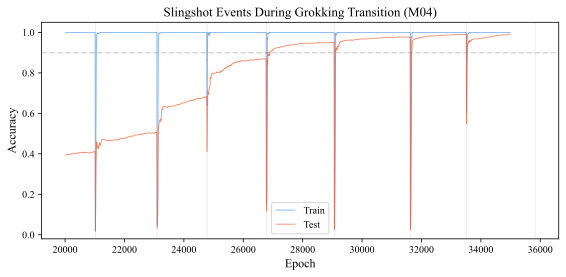
\includegraphics[width=0.92\textwidth]{figures/fig2_slingshots.png}
    \caption{Slingshot events during the grokking transition (epochs 20k--35k, M04). Red vertical lines mark 18 slingshot events---periodic train-accuracy collapses where the adaptive optimizer (AdamW) destabilizes the memorizing circuit.}
    \label{fig:slingshots}
\end{figure}

The slingshots follow the mechanism described by \citet{thilak2022slingshot}: adaptive optimizers at late stages of training exhibit cyclic phase transitions between stable and unstable regimes. In our setting, slingshot events \emph{coincide with and precede} the grokking transition. The final slingshot at epoch 26,780 (train accuracy drops from 1.0 to 0.15) is followed by test accuracy rising from $\sim$8\% to 93\% within 200 epochs. We do not claim that slingshots are \emph{necessary} for grokking---establishing necessity would require an intervention that eliminates slingshots and shows grokking disappears. Rather, we observe that slingshots consistently accompany the transition in our experiments.

\subsection{Weight Decay Schedule}

\begin{figure}[H]
    \centering
    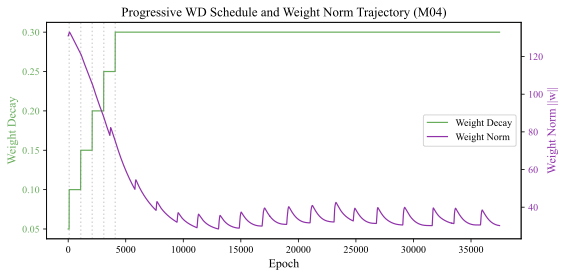
\includegraphics[width=0.90\textwidth]{figures/fig6_wd_schedule.png}
    \caption{Progressive weight decay schedule and weight norm trajectory (M04). WD ramps from 0.05 to 0.30 in steps of 0.05 every 1000 epochs after memorization. Weight norm decreases from 148 (initialization) to 30 (post-grokking).}
    \label{fig:wd_schedule}
\end{figure}

The WD schedule must satisfy three conditions for grokking:
\begin{enumerate}[leftmargin=*]
    \item \textbf{$\wdmax$ must be high enough} ($\geq 0.25$): With $\wdmax = 0.10$, the model never grokked even after 81k epochs.
    \item \textbf{WD ramp interval must be short} ($\leq 1000$ epochs): With $\Delta t_{\mathrm{ramp}} = 200{,}000$, WD never reached $\wdmax$ within the training budget.
    \item \textbf{Learning rate must not drop}: With \texttt{lr\_drop\_factor = 0.1}, the LR collapses to $10^{-8}$ after WD ramps, freezing the model. Setting \texttt{lr\_drop\_factor = 1.0} (no drop) is essential.
\end{enumerate}


% ============================================================================
% 7. MECHANISTIC ANALYSIS
% ============================================================================

\section{Mechanistic Analysis}
\label{sec:mechanistic}

\subsection{Group Structure Probes}

We probe checkpoints for group-theoretic structure. The discrete logarithm satisfies three key algebraic identities:
\begin{align}
    \textbf{Composition:} \quad & \log_g(h_1 \cdot h_2) = \log_g(h_1) + \log_g(h_2) \pmod{q} \\
    \textbf{Cyclic shift:} \quad & \log_g(g \cdot h) = \log_g(h) + 1 \pmod{q} \\
    \textbf{Inverse:} \quad & \log_g(h^{-1}) = -\log_g(h) \pmod{q}
\end{align}

\Cref{fig:group_structure} shows that group structure consistency rises \emph{in tandem} with test accuracy---the model is not merely memorizing input-output pairs but discovering the algebraic structure of the discrete logarithm.

\begin{figure}[H]
    \centering
    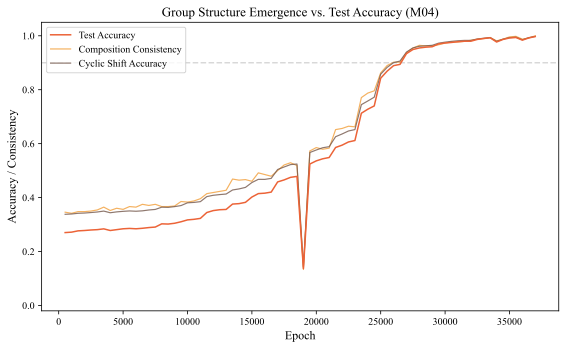
\includegraphics[width=0.90\textwidth]{figures/fig_group_structure.png}
    \caption{Group structure emergence vs. test accuracy (M04). Composition consistency and cyclic shift accuracy rise in tandem with test accuracy during the grokking transition.}
    \label{fig:group_structure}
\end{figure}

\subsection{Fourier Spectral Analysis}

We project hidden states onto both the multiplicative character basis $\{\chi_k\}$ and the additive character basis $\{\psi_k\}$. The multiplicative characters of $\Fps$ are naturally parameterized by discrete-log coordinates:
\begin{equation}
    \chi_k(h) = \exp\!\left(\frac{2\pi i \cdot k \cdot \log_g(h)}{q}\right), \quad k = 0, 1, \ldots, q-1,
\end{equation}
where $\log_g(h)$ is the discrete logarithm. The additive characters of $\Fp$ are:
\begin{equation}
    \psi_k(h) = \exp\!\left(\frac{2\pi i \cdot k \cdot h}{p}\right), \quad k = 0, 1, \ldots, p-1.
\end{equation}

\begin{figure}[H]
    \centering
    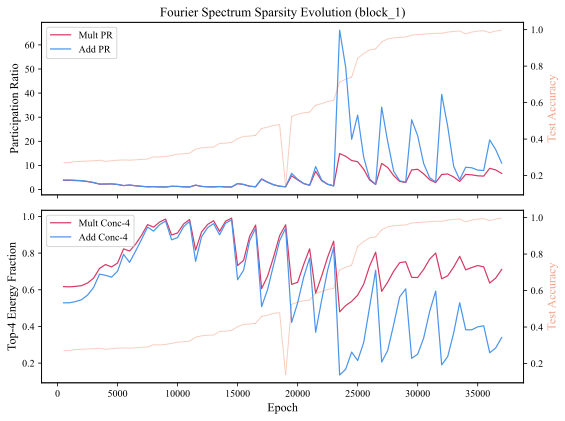
\includegraphics[width=0.94\textwidth]{figures/fig5_fourier_pr_evolution.png}
    \caption{Fourier spectrum sparsity evolution (M04, block\_1 layer). \textbf{Top:} Participation ratio for multiplicative and additive character bases, overlaid with test accuracy. \textbf{Bottom:} Top-4 energy concentration. A decrease in participation ratio indicates the model is developing a sparse Fourier representation.}
    \label{fig:fourier_pr}
\end{figure}

\Cref{fig:fourier_pr} shows that during grokking, the \emph{multiplicative} spectrum becomes increasingly sparse (participation ratio drops, top-4 concentration rises), while the additive spectrum remains relatively diffuse. This indicates the model's internal representation aligns with the multiplicative character basis---the natural Fourier basis for operations on $\Fps$ \citep{nguyen2026discrete}, since multiplicative characters are parameterized by discrete-log coordinates.

\subsection{Symbolic Regression as a Mechanistic Microscope}
\label{sec:symbolic}

\paragraph{Motivation.}
The Fourier analysis above shows that the model's representation is sparse in the multiplicative character basis. We now ask a stronger question: can symbolic regression (SR) discover explicit equations relating hidden states to the DLP solution? We apply SR as a \emph{mechanistic microscope} on the hidden states of the grokked M04 model, following the Cranmer-style symbolic distillation approach \citep{cranmer2020discovering}.

\paragraph{Setup.}
We extract activations from the pre-unembedding layer of the grokked M04 checkpoint across all 5,376 $(g, h)$ pairs. For each pair, we compute the analysis coordinates $g = g_0^a$, $h = g_0^b$, and the DLP solution $x = a^{-1} b \pmod{q}$. We then run PySR \citep{cranmer2023interpretable} on individual latent dimensions $z_j$ as a function of $(a, b)$, using two operator sets:
\begin{itemize}[leftmargin=*]
    \item \textbf{Free SR}: $+, -, \times, /, \sin, \cos, \exp, \log$---no modulo knowledge. This serves as an anti-leakage control.
    \item \textbf{Algebra-aware SR}: standard operators plus the precomputed modular features $a$, $b$, $a^{-1}$, $x$, $\cos(2\pi x/q)$, and $\sin(2\pi x/q)$.
\end{itemize}

\paragraph{Finding 1: Algebra-aware SR discovers multiplicative character structure.}
Algebra-aware SR preferentially selects $\cos(2\pi x/q)$ and $\sin(2\pi x/q)$ among the supplied modular features. These correspond to character coordinates after expressing group elements in DLP coordinates. The best fit achieves $R^2 = 0.42$ on dimension 54, compared to $R^2 = 0.04$ for free SR on the same dimension---a 9.7$\times$ improvement. Across 5 selected dimensions, algebra-aware SR achieves 3.3$\times$ higher mean $R^2$ than free SR.

\paragraph{Finding 2: Free SR independently discovers Fourier structure.}
Even without modulo knowledge, the free SR discovers Fourier-like structure: $\cos(b \cdot 1.5707)$ (where $1.5707 \approx \pi/2$) and $\sin(b \cdot 3.1206)$ (where $3.1206 \approx \pi$) appear repeatedly. For $q=112$, the recovered angular frequencies are close to valid Fourier harmonics: $\pi/2 = 2\pi(28)/112$ and $\pi = 2\pi(56)/112$. Thus the unconstrained search independently recovers harmonic structure without being given modular features.

\paragraph{Finding 3: Character structure is present throughout training.}
A temporal trajectory analysis across 12 checkpoints (epochs 499--37,481) on dimension 54 shows that $\cos(2\pi x / q)$ and $\sin(2\pi x / q)$ appear in the SR-discovered equations at \emph{every} checkpoint, including epoch 499 (post-memorization, pre-grokking). The correlation between the latent dimension and the DLP solution $x$ increases from 0.027 (epoch 499) to 0.066 (final), indicating that the character-based representation becomes more aligned with the DLP solution over training. Because this temporal analysis follows one selected dimension, we treat it as suggestive rather than definitive evidence: the character-aligned signal is detectable before generalization and changes during the grokking transition.

\begin{figure}[H]
    \centering
    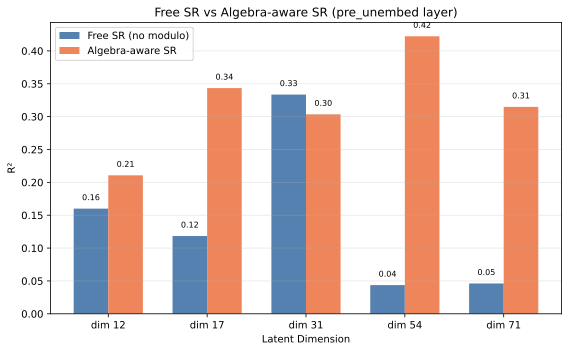
\includegraphics[width=0.86\textwidth]{figures/fig_sr_comparison.png}
    \caption{Free SR vs.\ algebra-aware SR on 5 latent dimensions (pre-unembedding layer, M04). Algebra-aware SR achieves 3.3$\times$ higher mean $R^2$ across these five dimensions, consistent with character-aligned structure in the hidden representation.}
    \label{fig:sr_comparison}
\end{figure}

\begin{figure}[H]
    \centering
    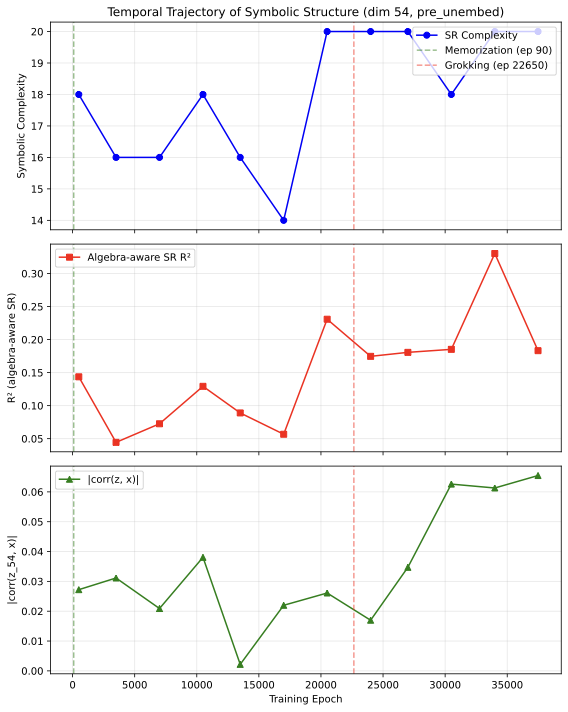
\includegraphics[width=0.82\textwidth]{figures/fig_sr_temporal.png}
    \caption{Temporal trajectory of symbolic structure (dimension 54, pre-unembedding layer). \textbf{Top:} SR complexity. \textbf{Middle:} Algebra-aware SR $R^2$. \textbf{Bottom:} Correlation between the latent dimension and the DLP solution $x$. Character-aligned features are detectable throughout this selected trajectory and change during grokking.}
    \label{fig:sr_temporal}
\end{figure}

\paragraph{Interpretation.}
The SR results are consistent with the spectral analysis: hidden states contain character-aligned trigonometric structure, and that structure evolves during training. The fact that free SR (without modulo knowledge) independently discovers Fourier structure provides an anti-leakage confirmation that the result is not an artifact of the algebra-aware operator set.


% ============================================================================
% 8. STRUCTURAL CONTROL: PRIME-ORDER DLP
% ============================================================================

\section{Structural Control: Prime-Order DLP}
\label{sec:prime_order}

\subsection{Motivation}

The DLP in $\Fps$ for $p = 113$ has group order $q = 112 = 16 \times 7$, which is smooth. This raises a natural concern: does grokking depend on the smooth factorization of $q$, perhaps exploiting CRT-like shortcuts? To test this, we study DLP in the order-113 subgroup of $\mathbb{F}_{227}^*$, where 113 is prime and no smooth factorization is available. This serves as a \emph{structural control}: if grokking still occurs, the phenomenon is not an artifact of smooth group structure.

\subsection{Results}

\begin{table}[H]
\centering
\caption{Prime-order DLP in the order-113 subgroup of $\mathbb{F}_{227}^*$. All experiments use 30\% training data. ``IID'' = random split, ``OOD'' = disjoint-generator split. Results from LUMI-G.}
\label{tab:prime_order_results}
\begin{tabular}{llrrrrrr}
\toprule
Model & Seed & Split & Best Acc & $\Tmem$ & $\Tninety$ & $\Tnine$ & Total Epochs \\
\midrule
M04 & 42 & IID & 100.0\% & 150 & 130,000 & 132,400 & 145,650 \\
M04 & 123 & IID & 100.0\% & 150 & 177,950 & 182,150 & 199,750 \\
M04 & 7 & IID & 99.99\% & 150 & 184,050 & 210,750 & 243,150 \\
M06 & 42 & IID & 100.0\% & 100 & 344,000 & 368,050 & 407,850 \\
M08 & 42 & IID & 99.90\% & 100 & 369,200 & 400,600 & 416,850 \\
M04 & 42 & OOD & 100.0\% & 200 & 236,100 & 254,950 & 326,150 \\
\bottomrule
\end{tabular}
\end{table}

\subsection{Key Findings}

\paragraph{DLP grokking is not restricted to smooth composite-order groups.}
All 6 experiments grok, including 3 seeds of M04 on the IID split. The model reaches near-perfect held-out accuracy in a prime-order group, where the short subgroup decompositions available at order 112 are absent.

\paragraph{The model generalizes to generators unseen during training.}
The OOD split (disjoint generators between train and test) groks at 100\% in 326K epochs. The model learns a mapping that transfers to generators not seen during training. We do not claim this proves a generator-independent algorithm without further mechanistic evidence.

\paragraph{Spectral analysis shows a different spectral profile.}
Extraction analysis of the grokked P113 model yields a decision-sufficient Fourier surrogate with 4 selected raw frequencies at 100\% argmax accuracy ($|K|/q = 4/113 = 3.5\%$), all with period 113 (no subgroup shortcuts). The spectral participation ratio is 96.0, compared to M04's 28.9 on the composite-order problem---a more diffuse representation adapted to the prime-order structure.

\begin{figure}[H]
    \centering
    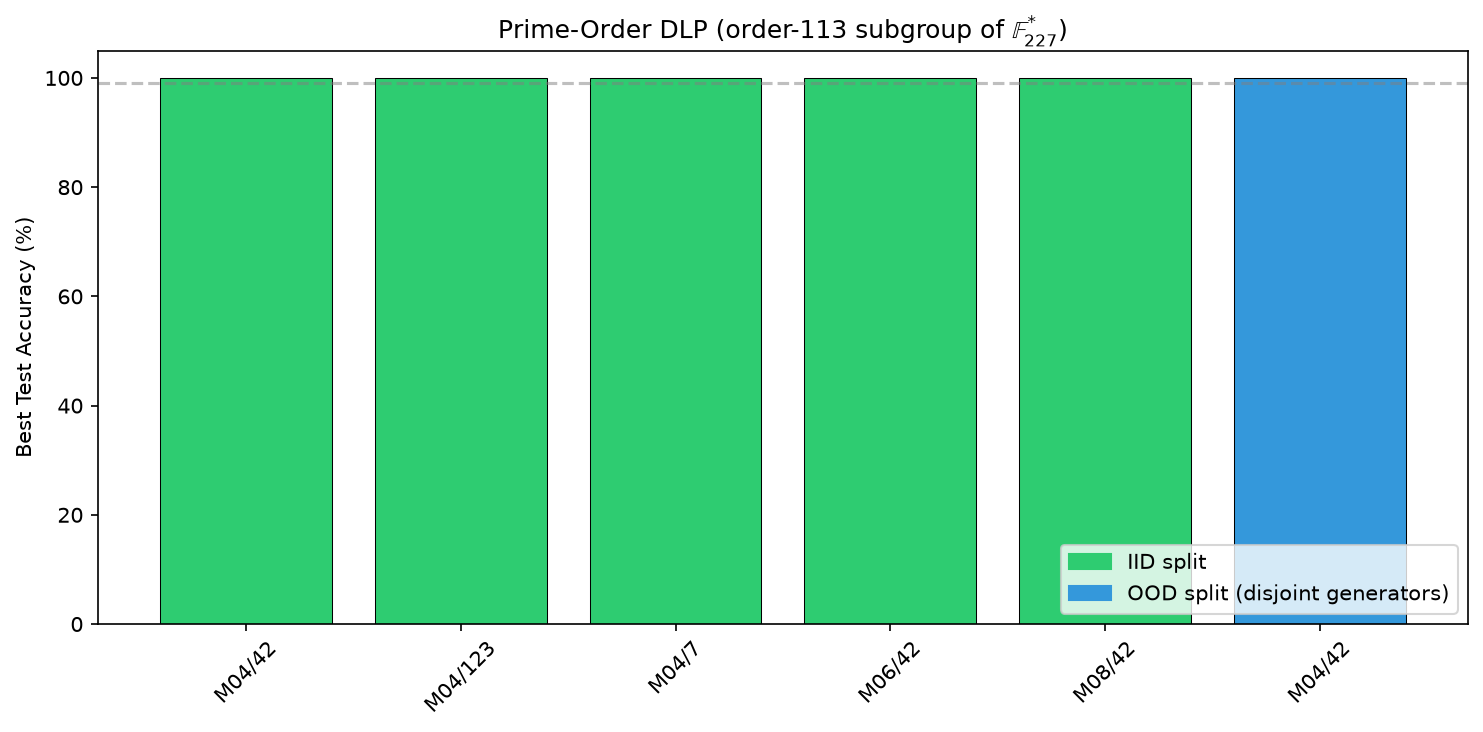
\includegraphics[width=0.88\textwidth]{figures/fig_prime_order.png}
    \caption{Prime-order DLP results from LUMI-G. All experiments grok, including the OOD (disjoint-generator) split. Green: IID split, Blue: OOD split.}
    \label{fig:lumi_prime_order}
\end{figure}


% ============================================================================
% 9. LIMITATIONS
% ============================================================================

\FloatBarrier
\section{Limitations}
\label{sec:limitations}

\begin{itemize}[leftmargin=*]
    \item \textbf{Modest mathematical scale.} The primary experiments use $p=113$, with a single extension check at $p=521$. These settings are useful for studying learning dynamics but do not support claims about practical cryptanalysis.

    \item \textbf{Capacity and data are partially entangled.} Training fraction changes across M07--M12. The sweep therefore demonstrates multi-scale grokking and a data-dependent non-monotonic region, but it is not a controlled one-variable scaling law.

    \item \textbf{Most capacity points are single-seed.} The prime-order control includes multiple seeds, but the main M01--M12 capacity sweep is primarily exploratory. Multi-seed replication is needed to estimate grokking probabilities near the empirical boundary.

    \item \textbf{Tokenizer growth with $p$.} The integer-token vocabulary expands with the field size, so the $p=521$ extension is not used to claim fixed-capacity problem-size scaling. A fixed-vocabulary study is better treated separately.

    \item \textbf{Optimization sensitivity.} The anchor result uses a progressive weight-decay schedule. Additional optimizer and regularization controls would be required to establish which training ingredients are causal rather than merely associated with grokking.

    \item \textbf{Symbolic regression is exploratory.} Fits to individual hidden dimensions remain moderate ($R^2$ up to 0.42). Stronger mechanistic claims require multi-dimensional symbolic models, exact full-domain verification, and causal intervention.

    \item \textbf{Compute normalization.} We report example presentations alongside epochs where available. Exact training FLOP accounting is implementation-dependent and is not used as a primary claim here.
\end{itemize}

% ============================================================================
% 10. DISCUSSION AND CONCLUSION
% ============================================================================

\FloatBarrier
\section{Discussion and Conclusion}
\label{sec:discussion}

\subsection{Why Does DLP Grok?}

Our observations are consistent with the circuit-efficiency framework \citep{varma2023explaining}. One plausible interpretation is that weight decay increasingly favors a lower-norm, structure-aligned solution over a memorizing solution. The spectral and symbolic analyses support the presence of multiplicative-character structure, but the present experiments do not establish a complete causal circuit.

\subsection{Open Questions}

Our results raise several questions for future work:
\begin{itemize}[leftmargin=*]
    \item Why does delayed generalization occur on this inverse problem, and what determines the grokking delay?
    \item How does the grokking boundary move under a fully matched capacity--data sweep with multiple seeds?
    \item Do the same representation transitions recur across model scales, or do larger models reach generalization by different internal routes?
    \item Does problem-size scaling eventually exceed the model's learnability frontier, and if so, where?
\end{itemize}

\subsection{Conclusion}

To the best of our knowledge, this work provides the first systematic demonstration of grokking on the full variable-base finite-field discrete logarithm mapping. A 427k-parameter transformer reaches 99.8\% held-out accuracy only after a long memorization phase, and the phenomenon reappears across a 12-model sweep extending to 14.4M parameters. The sweep also reveals a non-monotonic, data-dependent region, emphasizing that neural scale alone does not determine whether grokking occurs. Mechanistic analyses show that successful generalization is accompanied by multiplicative-character/Fourier structure, with symbolic regression independently recovering harmonic features from hidden states. Prime-order and disjoint-generator controls further show that successful generalization is not confined to the smooth order-112 setting. Together, these results establish DLP as a compact but nontrivial benchmark for studying how neural networks transition from memorization to structured generalization across model scale.

\subsection*{Data and Code Availability}
The mathematical datasets in this study are deterministically generated from the task definitions. The exact split manifests, run-level metrics, figure source data, model configurations, training code, and analysis code are publicly available at \url{https://github.com/VesterlundCoder/dlp-grokking}. An archival DOI with frozen code snapshot, split manifests, and selected checkpoints will be deposited at release.

% ============================================================================
% REFERENCES
% ============================================================================

\begin{thebibliography}{99}
\bibitem[Power et~al.(2022)]{power2022grokking} Power, A., Burda, Y., Edwards, H., Babuschkin, I., and Misra, V. (2022). Grokking: Generalization Beyond Overfitting on Small Algorithmic Datasets. \emph{ICLR}.
\bibitem[Nanda et~al.(2023)]{nanda2023progress} Nanda, N., Chan, L., Lieberum, T., Smith, J., and Steinhardt, J. (2023). Progress Measures for Grokking via Mechanistic Interpretability. \emph{ICLR}.
\bibitem[Liu et~al.(2022)]{liu2022understanding} Liu, Z., Kitouni, O., Nolte, N., Michaud, E. J., Tegmark, M., and Williams, M. (2022). Towards Understanding Grokking: An Effective Theory of Representation Learning. \emph{NeurIPS}.
\bibitem[Varma et~al.(2023)]{varma2023explaining} Varma, V., Davies, W., et al. (2023). Explaining Grokking Through Circuit Efficiency. arXiv:2309.02390.
\bibitem[Thilak et~al.(2022)]{thilak2022slingshot} Thilak, N., Lai, E., Goh, L., Wattenberg, M., et al. (2022). The Slingshot Mechanism: An Empirical Study of Adaptive Optimizers and the Grokking Phenomenon. arXiv:2206.04817.
\bibitem[Takhanov et~al.(2024)]{takhanov2024intractability} Takhanov, R., Tezekbayev, M., Pak, A., Bolatov, A., Kadyrsizova, Z., and Assylbekov, Z. (2024). Intractability of Learning the Discrete Logarithm with Gradient-Based Methods. \emph{Proceedings of Machine Learning Research}, 222.
\bibitem[Nguyen(2026)]{nguyen2026discrete} Nguyen, H. D. (2026). The Discrete-Log Clock: How a Transformer Learns Modular Multiplication. arXiv:2606.17399.
\bibitem[Cranmer et~al.(2020)]{cranmer2020discovering} Cranmer, M., Sanchez-Gonzalez, A., Battaglia, P., Xu, R., Cranmer, K., Spergel, D., and Ho, S. (2020). Discovering Symbolic Models from Deep Learning with Inductive Biases. \emph{NeurIPS} 33.
\bibitem[Cranmer(2023)]{cranmer2023interpretable} Cranmer, M. (2023). Interpretable Machine Learning for Science with PySR and SymbolicRegression.jl. arXiv:2305.01582.
\bibitem[Loshchilov and Hutter(2019)]{loshchilov2019decoupled} Loshchilov, I. and Hutter, F. (2019). Decoupled Weight Decay Regularization. \emph{ICLR}.
\bibitem[Vaswani et~al.(2017)]{vaswani2017attention} Vaswani, A., Shazeer, N., Parmar, N., Uszkoreit, J., Jones, L., Gomez, A. N., Kaiser, L., and Polosukhin, I. (2017). Attention Is All You Need. \emph{NeurIPS}.
\end{thebibliography}

\end{document}
